% !TEX TS-program = pdflatex
\documentclass[11pt]{article}

% -------------------- Packages --------------------
\usepackage[a4paper,margin=1in]{geometry}
\usepackage{amsmath,amssymb}
\usepackage[T1]{fontenc}
\usepackage{lmodern}
\usepackage{xcolor}
\usepackage{tcolorbox}
\tcbuselibrary{skins,breakable}
\usepackage{enumitem}
\usepackage{hyperref}
\usepackage{tikz}
\usetikzlibrary{calc,arrows.meta}

\pagestyle{empty}

% -------------------- Dark Theme Colors --------------------
\definecolor{bg}{HTML}{000000}
\definecolor{pairbg}{HTML}{121212}
\definecolor{solbg}{HTML}{0A0A0A}
\definecolor{border}{HTML}{2A2A2A}
\definecolor{text}{HTML}{FFFFFF}
\definecolor{muted}{HTML}{C9CDD3}
\definecolor{gold}{HTML}{FFD700}
\definecolor{green}{HTML}{4ADE80}
\definecolor{cyan}{HTML}{38BDF8}

\pagecolor{bg}
\color{text}

\hypersetup{
  colorlinks=true,
  linkcolor=cyan,
  urlcolor=cyan
}

\setlength{\parindent}{0pt}
\setlength{\parskip}{10pt}

\setlist[itemize]{left=1.4em,itemsep=6pt,topsep=6pt}
\setlist[enumerate]{left=1.6em,itemsep=4pt,topsep=4pt}

% -------------------- tcolorbox Base --------------------
\tcbset{
  enhanced,
  breakable,
  arc=12pt,
  boxrule=0.8pt,
  left=16pt,right=16pt,top=12pt,bottom=12pt
}

\newtcolorbox{QAPair}[1]{%
  colback=pairbg,
  colbacklower=solbg,
  colframe=border,
  coltext=text,
  title=\textcolor{gold}{\bfseries #1},
  fonttitle=\bfseries,
  coltitle=text,
  segmentation style={draw=border, dashed, line width=0.6pt},
}

\newtcolorbox{QuickBox}{%
  colback=pairbg,
  colframe=cyan,
  coltext=text,
  fontupper=\color{text},
  borderline north={4pt}{0pt}{cyan},
  arc=14pt,
  boxrule=0.8pt
}

% Helper for step headings
\newcommand{\Step}[1]{\textcolor{muted}{\textbf{Step #1:}}}

% Vector helpers
\newcommand{\ii}{\mathbf{i}}
\newcommand{\jj}{\mathbf{j}}
\newcommand{\pos}[1]{\overrightarrow{O#1}}
\newcommand{\vv}[1]{\overrightarrow{#1}}

% Small coordinate-plane helper
\newcommand{\Axes}[4]{%
  \draw[->,color=text] (#1,0) -- (#2,0) node[right,color=text] {$x$};
  \draw[->,color=text] (0,#3) -- (0,#4) node[above,color=text] {$y$};
  \draw[color=border, step=1cm] (#1,#3) grid (#2,#4);
}

% ============================================================
\begin{document}

\begin{center}
{\LARGE\bfseries \textcolor{gold}{Exercise 7.2 --- Solutions}}\\[-2pt]
\end{center}

\begin{QuickBox}
{\color{cyan}\bfseries Quick formulas (vectors \& coordinate geometry)}\par\medskip
\begin{itemize}
\item \textbf{Position vector:} if $A(x,y)$ then $\pos{A}=x\ii+y\jj$.
\item \textbf{Displacement vector:} $\vv{AB}=\pos{B}-\pos{A}$.
\item \textbf{Length:} if $\vec{v}=a\ii+b\jj$, then $|\vec{v}|=\sqrt{a^2+b^2}$.
\item \textbf{Midpoint:} $M\left(\dfrac{x_1+x_2}{2},\dfrac{y_1+y_2}{2}\right)$.
\item \textbf{Section formula (internal):} if $P$ divides $AB$ in ratio $m:n$ (i.e.\ $AP:PB=m:n$), then
\[
\pos{P}=\frac{n\pos{A}+m\pos{B}}{m+n}.
\]
\item \textbf{Parallelogram:} diagonals $\vec{d}_1=\vec{a}+\vec{b}$ and $\vec{d}_2=\vec{a}-\vec{b}$ (adjacent sides $\vec{a},\vec{b}$).
\end{itemize}
\end{QuickBox}

% ============================================================
\begin{QAPair}{Question 1}
\textcolor{gold}{\bfseries Question:} What type of quadrilateral $EFGH$ is it if $\vv{EF}=\vv{HG}$ and $\vv{EH}=\vv{FG}$?\\
\tcblower
\textcolor{green}{\bfseries Answer:}
\[
\begin{aligned}
\Step{1}\;& \vv{EF}=\vv{HG}\ \Rightarrow\ EF \parallel HG \text{ and } EF=HG.\\
\Step{2}\;& \vv{EH}=\vv{FG}\ \Rightarrow\ EH \parallel FG \text{ and } EH=FG.\\
\Step{3}\;& \text{Both pairs of opposite sides are parallel } \Rightarrow EFGH \text{ is a parallelogram.}
\end{aligned}
\]
\[
\boxed{\text{$EFGH$ is a \textbf{parallelogram}.}}
\]
\end{QAPair}

% ============================================================
\begin{QAPair}{Question 2}
\textcolor{gold}{\bfseries Question:} Use vectors to find the lengths of diagonals of a parallelogram having adjacent sides $2\ii+\jj$ and $\ii-3\jj$.\\
\tcblower
\textcolor{green}{\bfseries Answer:}
Let $\vec{a}=2\ii+\jj$ and $\vec{b}=\ii-3\jj$.
\[
\begin{aligned}
\Step{1}\;& \text{Diagonals are } \vec{d}_1=\vec{a}+\vec{b},\ \vec{d}_2=\vec{a}-\vec{b}.\\
\Step{2}\;& \vec{d}_1=(2\ii+\jj)+(\ii-3\jj)=3\ii-2\jj
\ \Rightarrow\ |\vec{d}_1|=\sqrt{3^2+(-2)^2}=\sqrt{13}.\\
\Step{3}\;& \vec{d}_2=(2\ii+\jj)-(\ii-3\jj)=\ii+4\jj
\ \Rightarrow\ |\vec{d}_2|=\sqrt{1^2+4^2}=\sqrt{17}.
\end{aligned}
\]
\[
\boxed{\text{Diagonal lengths are } \sqrt{13}\ \text{and}\ \sqrt{17}.}
\]
\end{QAPair}

% ============================================================
\begin{QAPair}{Question 3 (i)}
\textcolor{gold}{\bfseries Question:} Show that $A(0,2)$, $B(\sqrt3,-1)$, $C(0,-2)$ are vertices of a right-angled triangle.\\
\tcblower
\textcolor{green}{\bfseries Answer:}
\[
\begin{aligned}
\Step{1}\;& AB^2=(\sqrt3-0)^2+(-1-2)^2=3+9=12.\\
\Step{2}\;& BC^2=(0-\sqrt3)^2+(-2+1)^2=3+1=4.\\
\Step{3}\;& AC^2=(0-0)^2+(-2-2)^2=16.\\
\Step{4}\;& AB^2+BC^2=12+4=16=AC^2.
\end{aligned}
\]
So by Pythagoras, the triangle is right-angled at $B$.
\[
\boxed{\angle ABC=90^\circ.}
\]

\textcolor{muted}{\textbf{Diagram (not to scale):}}
\begin{center}
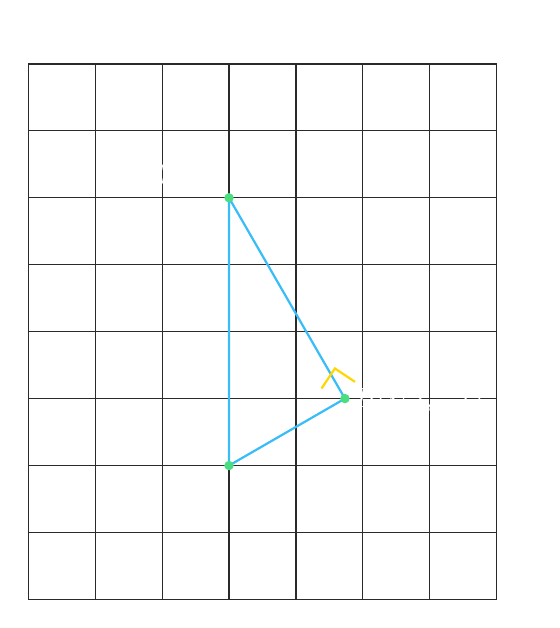
\begin{tikzpicture}[scale=0.85]
  \Axes{-3}{4}{-4}{4}
  \coordinate (A) at (0,2);
  \coordinate (B) at ({sqrt(3)},-1);
  \coordinate (C) at (0,-2);
  \draw[thick,color=cyan] (A)--(B)--(C)--cycle;
  \fill[color=green] (A) circle (2pt) node[above left,color=text] {$A(0,2)$};
  \fill[color=green] (B) circle (2pt) node[right,color=text] {$B(\sqrt3,-1)$};
  \fill[color=green] (C) circle (2pt) node[below left,color=text] {$C(0,-2)$};
  % right angle marker at B
  \draw[color=gold,thick] ($(B)+(-0.35,0.15)$) -- ($(B)+(-0.15,0.45)$) -- ($(B)+(0.15,0.25)$);
\end{tikzpicture}
\end{center}
\end{QAPair}

% ============================================================
\begin{QAPair}{Question 3 (ii)}
\textcolor{gold}{\bfseries Question:} Show that $A(3,1)$, $B(-2,-3)$, $C(2,2)$ are vertices of an isosceles triangle.\\
\tcblower
\textcolor{green}{\bfseries Answer:}
\[
\begin{aligned}
\Step{1}\;& AB^2=(-2-3)^2+(-3-1)^2=25+16=41.\\
\Step{2}\;& BC^2=(2+2)^2+(2+3)^2=16+25=41.\\
\Step{3}\;& AB^2=BC^2 \Rightarrow AB=BC.
\end{aligned}
\]
\[
\boxed{\text{Triangle } ABC \text{ is isosceles with } AB=BC\ \text{(base } AC\text{).}}
\]

\textcolor{muted}{\textbf{Diagram (not to scale):}}
\begin{center}
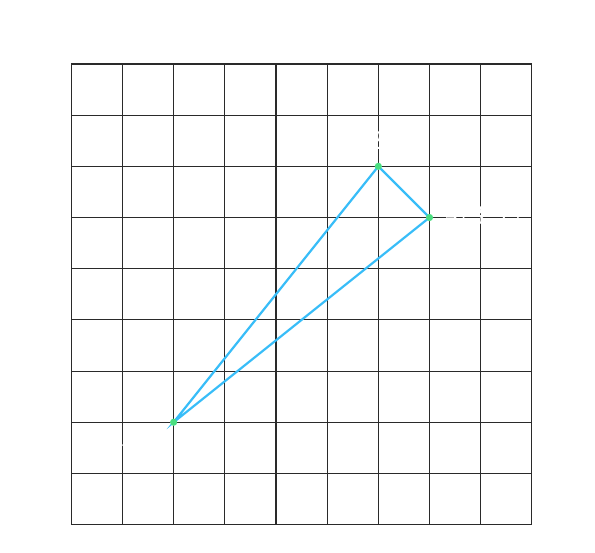
\begin{tikzpicture}[scale=0.65]
  \Axes{-4}{5}{-5}{4}
  \coordinate (A) at (3,1);
  \coordinate (B) at (-2,-3);
  \coordinate (C) at (2,2);
  \draw[thick,color=cyan] (A)--(B)--(C)--cycle;
  \fill[color=green] (A) circle (2pt) node[right,color=text] {$A(3,1)$};
  \fill[color=green] (B) circle (2pt) node[below left,color=text] {$B(-2,-3)$};
  \fill[color=green] (C) circle (2pt) node[above,color=text] {$C(2,2)$};
\end{tikzpicture}
\end{center}
\end{QAPair}

% ============================================================
\begin{QAPair}{Question 4}
\textcolor{gold}{\bfseries Question:} The position vectors of $C$ and $D$ are $3\ii+2\jj$ and $\ii-4\jj$ respectively. Find the position vector of point $O$ dividing $CD$ in the ratio $2:3$ internally.\\
\tcblower
\textcolor{green}{\bfseries Answer:}
Let $\pos{C}=3\ii+2\jj$ and $\pos{D}=\ii-4\jj$. If $CO:OD=2:3$, then
\[
\begin{aligned}
\Step{1}\;& \pos{O}=\frac{3\pos{C}+2\pos{D}}{2+3}.\\
\Step{2}\;& 3\pos{C}=9\ii+6\jj,\quad 2\pos{D}=2\ii-8\jj.\\
\Step{3}\;& \pos{O}=\frac{(9\ii+6\jj)+(2\ii-8\jj)}{5}
=\frac{11\ii-2\jj}{5}.
\end{aligned}
\]
\[
\boxed{\pos{O}=\frac{11}{5}\ii-\frac{2}{5}\jj.}
\]
\end{QAPair}

% ============================================================
\begin{QAPair}{Question 5}
\textcolor{gold}{\bfseries Question:} If $M(2,4)$ is the mid-point of $XY$ such that $X(-1,3)$ and $Y(x,y)$. Find the point $Y$.\\
\tcblower
\textcolor{green}{\bfseries Answer:}
\[
\begin{aligned}
\Step{1}\;& \left(\frac{-1+x}{2},\frac{3+y}{2}\right)=(2,4).\\
\Step{2}\;& \frac{-1+x}{2}=2 \Rightarrow -1+x=4 \Rightarrow x=5.\\
\Step{3}\;& \frac{3+y}{2}=4 \Rightarrow 3+y=8 \Rightarrow y=5.
\end{aligned}
\]
\[
\boxed{Y(5,5).}
\]
\end{QAPair}

% ============================================================
\begin{QAPair}{Question 6}
\textcolor{gold}{\bfseries Question:} If $\pos{A}=2\ii+3\jj$, $\pos{B}=6\ii+2\jj$, find the point(s) trisecting the join of $AB$.\\
\tcblower
\textcolor{green}{\bfseries Answer:}
Trisection points divide $AB$ internally in ratios $1:2$ and $2:1$.

\[
\begin{aligned}
\Step{1}\;& P:\ AP:PB=1:2 \Rightarrow \pos{P}=\frac{2\pos{A}+1\pos{B}}{3}.\\
&\pos{A}=(2,3),\ \pos{B}=(6,2)\Rightarrow
P=\left(\frac{2\cdot2+6}{3},\frac{2\cdot3+2}{3}\right)=\left(\frac{10}{3},\frac{8}{3}\right).\\[4pt]
\Step{2}\;& Q:\ AQ:QB=2:1 \Rightarrow \pos{Q}=\frac{1\pos{A}+2\pos{B}}{3}.\\
&Q=\left(\frac{2+2\cdot6}{3},\frac{3+2\cdot2}{3}\right)=\left(\frac{14}{3},\frac{7}{3}\right).
\end{aligned}
\]
\[
\boxed{P\left(\frac{10}{3},\frac{8}{3}\right),\quad Q\left(\frac{14}{3},\frac{7}{3}\right).}
\]
\end{QAPair}

% ============================================================
\begin{QAPair}{Question 7}
\textcolor{gold}{\bfseries Question:} Find $x$ such that the points $P(-1,x)$, $Q(3,2)$ and $R(7,3)$ are collinear.\\
\tcblower
\textcolor{green}{\bfseries Answer:}
For collinearity, slopes must be equal.
\[
\begin{aligned}
\Step{1}\;& \text{slope } QR=\frac{3-2}{7-3}=\frac{1}{4}.\\
\Step{2}\;& \text{slope } PQ=\frac{2-x}{3-(-1)}=\frac{2-x}{4}.\\
\Step{3}\;& \frac{2-x}{4}=\frac{1}{4}\Rightarrow 2-x=1\Rightarrow x=1.
\end{aligned}
\]
\[
\boxed{x=1.}
\]
\end{QAPair}

% ============================================================
\begin{QAPair}{Question 8}
\textcolor{gold}{\bfseries Question:} Find the coordinates of vertex $D$ of a parallelogram $ABCD$ if $A(-3,0)$, $B(1,-2)$ and $C(5,0)$ are its three vertices.\\
\tcblower
\textcolor{green}{\bfseries Answer:}
In a parallelogram (with vertices in order), $\pos{A}+\pos{C}=\pos{B}+\pos{D}$.
\[
\begin{aligned}
\Step{1}\;& D=A+C-B.\\
\Step{2}\;& A(-3,0),\ C(5,0),\ B(1,-2)\\
&\Rightarrow D=(-3+5-1,\ 0+0-(-2))=(1,2).
\end{aligned}
\]
\[
\boxed{D(1,2).}
\]
\end{QAPair}

% ============================================================
\begin{QAPair}{Question 9}
\textcolor{gold}{\bfseries Question:} If $\vv{AB}=\vv{CD}$ and $A(0,2)$, $C(-2,4)$, $D(-1,5)$, then find vertex $B$.\\
\tcblower
\textcolor{green}{\bfseries Answer:}
\[
\begin{aligned}
\Step{1}\;& \vv{CD}=D-C=\bigl((-1)-(-2),\ 5-4\bigr)=(1,1).\\
\Step{2}\;& \vv{AB}=\vv{CD}\Rightarrow B=A+\vv{CD}.\\
\Step{3}\;& B=(0,2)+(1,1)=(1,3).
\end{aligned}
\]
\[
\boxed{B(1,3).}
\]
\end{QAPair}

% ============================================================
\begin{QAPair}{Question 10}
\textcolor{gold}{\bfseries Question:} Vertices of a quadrilateral are $U(9,4)$, $V(-7,7)$, $W(-4,-7)$ and $X(5,-5)$. Find midpoints of its sides and prove that the figure obtained by joining midpoints consecutively is a parallelogram.\\
\tcblower
\textcolor{green}{\bfseries Answer:}
Let midpoints be
\[
\begin{aligned}
\Step{1}\;& M=\text{midpoint of }UV=\left(\frac{9+(-7)}{2},\frac{4+7}{2}\right)=\left(1,\frac{11}{2}\right).\\
\Step{2}\;& N=\text{midpoint of }VW=\left(\frac{-7+(-4)}{2},\frac{7+(-7)}{2}\right)=\left(-\frac{11}{2},0\right).\\
\Step{3}\;& P=\text{midpoint of }WX=\left(\frac{-4+5}{2},\frac{-7+(-5)}{2}\right)=\left(\frac12,-6\right).\\
\Step{4}\;& Q=\text{midpoint of }XU=\left(\frac{5+9}{2},\frac{-5+4}{2}\right)=\left(7,-\frac12\right).
\end{aligned}
\]
Now check opposite sides:
\[
\begin{aligned}
\Step{5}\;& \vv{MN}=N-M=\left(-\frac{11}{2}-1,\ 0-\frac{11}{2}\right)=\left(-\frac{13}{2},-\frac{11}{2}\right).\\
\Step{6}\;& \vv{PQ}=Q-P=\left(7-\frac12,\ -\frac12-(-6)\right)=\left(\frac{13}{2},\frac{11}{2}\right)=-\vv{MN}.\\
\Step{7}\;& \Rightarrow MN \parallel PQ \text{ and } MN=PQ.\\[4pt]
\Step{8}\;& \vv{NP}=P-N=\left(\frac12+\frac{11}{2},\ -6-0\right)=(6,-6).\\
\Step{9}\;& \vv{MQ}=Q-M=\left(7-1,\ -\frac12-\frac{11}{2}\right)=(6,-6)=\vv{NP}.\\
\Step{10}\;& \Rightarrow NP \parallel MQ \text{ and } NP=MQ.
\end{aligned}
\]
Hence, $MNPQ$ is a parallelogram.
\[
\boxed{M\left(1,\frac{11}{2}\right),\ N\left(-\frac{11}{2},0\right),\ P\left(\frac12,-6\right),\ Q\left(7,-\frac12\right);\ \text{and } MNPQ \text{ is a parallelogram.}}
\]

\textcolor{muted}{\textbf{Diagram (midpoint quadrilateral):}}
\begin{center}
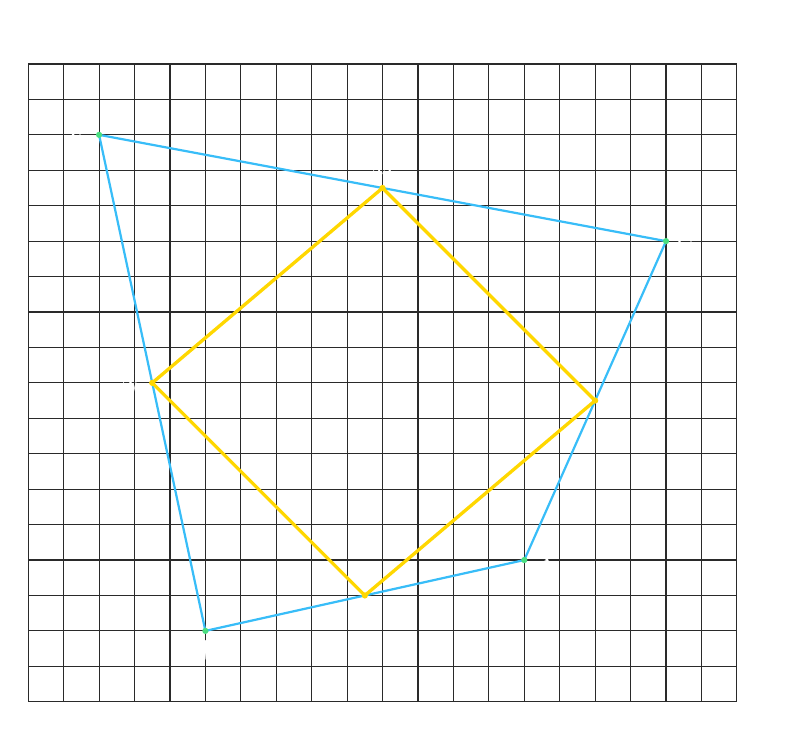
\begin{tikzpicture}[scale=0.45]
  \Axes{-9}{11}{-9}{9}
  \coordinate (U) at (9,4);
  \coordinate (V) at (-7,7);
  \coordinate (W) at (-4,-7);
  \coordinate (X) at (5,-5);

  \coordinate (M) at (1,5.5);
  \coordinate (N) at (-5.5,0);
  \coordinate (P) at (0.5,-6);
  \coordinate (Q) at (7,-0.5);

  \draw[thick,color=cyan] (U)--(V)--(W)--(X)--cycle;
  \draw[very thick,color=gold] (M)--(N)--(P)--(Q)--cycle;

  \fill[color=green] (U) circle (2.5pt) node[right,color=text] {$U$};
  \fill[color=green] (V) circle (2.5pt) node[left,color=text] {$V$};
  \fill[color=green] (W) circle (2.5pt) node[below,color=text] {$W$};
  \fill[color=green] (X) circle (2.5pt) node[right,color=text] {$X$};

  \fill[color=gold] (M) circle (2.5pt) node[above,color=text] {$M$};
  \fill[color=gold] (N) circle (2.5pt) node[left,color=text] {$N$};
  \fill[color=gold] (P) circle (2.5pt) node[below,color=text] {$P$};
  \fill[color=gold] (Q) circle (2.5pt) node[right,color=text] {$Q$};
\end{tikzpicture}
\end{center}
\end{QAPair}

% ============================================================
\begin{QAPair}{Question 11}
\textcolor{gold}{\bfseries Question:} Prove that the line segment joining the midpoints of two sides of a triangle is half in length of the third side.\\
\tcblower
\textcolor{green}{\bfseries Answer (vector proof):}
Let triangle be $ABC$ with position vectors $\pos{A}=\vec{a}$, $\pos{B}=\vec{b}$, $\pos{C}=\vec{c}$.
Let $D$ be midpoint of $AB$ and $E$ be midpoint of $AC$.
\[
\begin{aligned}
\Step{1}\;& \pos{D}=\frac{\vec{a}+\vec{b}}{2},\quad \pos{E}=\frac{\vec{a}+\vec{c}}{2}.\\
\Step{2}\;& \vv{DE}=\pos{E}-\pos{D}
=\frac{\vec{a}+\vec{c}}{2}-\frac{\vec{a}+\vec{b}}{2}
=\frac{\vec{c}-\vec{b}}{2}.\\
\Step{3}\;& \vv{BC}=\vec{c}-\vec{b}\Rightarrow \vv{DE}=\frac{1}{2}\vv{BC}.
\end{aligned}
\]
So $DE\parallel BC$ and $|DE|=\dfrac{1}{2}|BC|$.
\[
\boxed{|DE|=\frac{1}{2}|BC|\ \text{(and } DE\parallel BC\text{).}}
\]
\end{QAPair}

% ============================================================
\begin{QAPair}{Question 12}
\textcolor{gold}{\bfseries Question:} Prove that the joining the midpoints of the two non-parallel sides of a trapezium is parallel to its parallel sides.\\
\tcblower
\textcolor{green}{\bfseries Answer (vector proof):}
Let $ABCD$ be a trapezium with $AB\parallel CD$ and non-parallel sides $AD$ and $BC$.
Let $M$ be midpoint of $AD$ and $N$ midpoint of $BC$.
\[
\begin{aligned}
\Step{1}\;& \pos{M}=\frac{\pos{A}+\pos{D}}{2},\quad \pos{N}=\frac{\pos{B}+\pos{C}}{2}.\\
\Step{2}\;& \vv{MN}=\pos{N}-\pos{M}
=\frac{\pos{B}+\pos{C}-\pos{A}-\pos{D}}{2}\\
&=\frac{(\pos{B}-\pos{A})+(\pos{C}-\pos{D})}{2}
=\frac{\vv{AB}+\vv{DC}}{2}.
\end{aligned}
\]
\[
\Step{3}\; AB\parallel CD \Rightarrow \vv{DC} \text{ is parallel to } \vv{AB}.
\]
Hence $\vv{MN}$ is a scalar multiple of a vector parallel to $\vv{AB}$, so $MN\parallel AB$ (and also $MN\parallel CD$).
\[
\boxed{MN\parallel AB\parallel CD.}
\]
\end{QAPair}

% ============================================================
\begin{QAPair}{Question 13}
\textcolor{gold}{\bfseries Question:} Prove that the line segment joining midpoints of adjacent sides of a square/rectangle/parallelogram divides the corresponding diagonal in the ratio $1:3$.\\
\tcblower
\textcolor{green}{\bfseries Answer (parallelogram proof; square/rectangle are special cases):}

Let $ABCD$ be a parallelogram. Take $A$ as origin.
Let $\vv{AB}=\vec{b}$ and $\vv{AD}=\vec{d}$. Then
\[
\pos{A}=\vec{0},\quad \pos{B}=\vec{b},\quad \pos{D}=\vec{d},\quad \pos{C}=\vec{b}+\vec{d}.
\]
Let $M$ be midpoint of $AB$ and $N$ be midpoint of $AD$.
\[
\begin{aligned}
\Step{1}\;& \pos{M}=\frac{\pos{A}+\pos{B}}{2}=\frac{\vec{b}}{2},\qquad
\pos{N}=\frac{\pos{A}+\pos{D}}{2}=\frac{\vec{d}}{2}.\\
\Step{2}\;& \text{Line } MN:\ \pos{R}=\pos{M}+t(\pos{N}-\pos{M})
=\frac{\vec{b}}{2}+t\left(\frac{\vec{d}-\vec{b}}{2}\right).\\
\Step{3}\;& \text{Diagonal } AC:\ \pos{S}=s(\vec{b}+\vec{d}).
\end{aligned}
\]
At the intersection point $P$, $\pos{R}=\pos{S}$, so
\[
\frac{\vec{b}}{2}+t\left(\frac{\vec{d}-\vec{b}}{2}\right)=s(\vec{b}+\vec{d})
\Rightarrow \frac{(1-t)}{2}\vec{b}+\frac{t}{2}\vec{d}=s\vec{b}+s\vec{d}.
\]
Comparing coefficients of $\vec{b}$ and $\vec{d}$:
\[
\frac{1-t}{2}=s,\qquad \frac{t}{2}=s \Rightarrow 1-t=t \Rightarrow t=\frac12,\quad s=\frac14.
\]
So $P$ divides diagonal $AC$ with
\[
\pos{P}=\frac14(\vec{b}+\vec{d}) \Rightarrow AP=\frac14 AC,\quad PC=\frac34 AC.
\]
\[
\boxed{AP:PC=1:3.}
\]
Since a square and rectangle are parallelograms, the result holds for them as well.

\textcolor{muted}{\textbf{Diagram (generic parallelogram):}}
\begin{center}
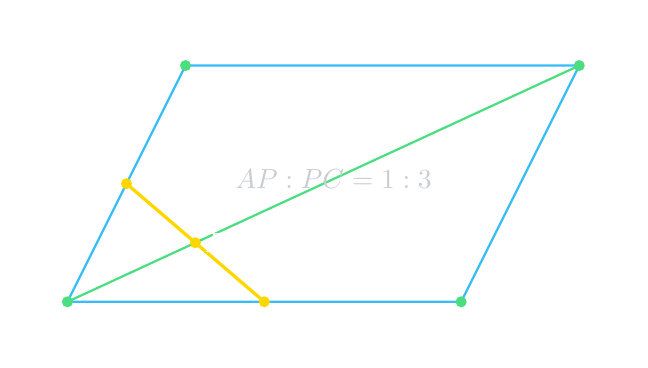
\begin{tikzpicture}[scale=1.0]
  \coordinate (A) at (0,0);
  \coordinate (B) at (5,0);
  \coordinate (D) at (1.5,3);
  \coordinate (C) at ($(B)+(D)-(A)$);

  \coordinate (M) at ($(A)!0.5!(B)$);
  \coordinate (N) at ($(A)!0.5!(D)$);
  \coordinate (P) at ($(A)!0.25!(C)$);

  \draw[thick,color=cyan] (A)--(B)--(C)--(D)--cycle;
  \draw[thick,color=green] (A)--(C);
  \draw[very thick,color=gold] (M)--(N);

  \fill[color=green] (A) circle (2pt) node[below left,color=text] {$A$};
  \fill[color=green] (B) circle (2pt) node[below,color=text] {$B$};
  \fill[color=green] (C) circle (2pt) node[above right,color=text] {$C$};
  \fill[color=green] (D) circle (2pt) node[above,color=text] {$D$};

  \fill[color=gold] (M) circle (2pt) node[below,color=text] {$M$};
  \fill[color=gold] (N) circle (2pt) node[left,color=text] {$N$};
  \fill[color=gold] (P) circle (2pt) node[right,color=text] {$P$};

  \node[color=muted] at ($(A)!0.52!(C)$) {$AP:PC=1:3$};
\end{tikzpicture}
\end{center}
\end{QAPair}

\end{document}
